%!TEX root = ./main.tex

%%**************************************************************
%%
%% DHBW Heidenheim - Template for Bachelor Thesis
%%
%% Bevor usisng this template please have a look at the REAMDME.md file
%%
%%**************************************************************

%!TEX root = ../dokumentation.tex

%
% Nahezu alle Einstellungen koennen hier getaetigt werden
%

\RequirePackage[l2tabu, orthodox]{nag}	% weist in Commandozeile bzw. log auf veraltete LaTeX Syntax hin

\documentclass[%
	pdftex,
	oneside,			% Einseitiger Druck.
	12pt,				% Schriftgroesse
	parskip=half,		% Halbe Zeile Abstand zwischen Absätzen.
%	topmargin = 10pt,	% Abstand Seitenrand (Std:1in) zu Kopfzeile [laut log: unused]
	headheight = 12pt,	% Höhe der Kopfzeile
%	headsep = 30pt,	% Abstand zwischen Kopfzeile und Text Body  [laut log: unused]
	headsepline,		% Linie nach Kopfzeile.
	footsepline,		% Linie vor Fusszeile.
	footheight = 16pt,	% Höhe der Fusszeile
	abstracton,		% Abstract Überschriften
	DIV=calc,		% Satzspiegel berechnen
	BCOR=8mm,		% Bindekorrektur links: 8mm
	headinclude=false,	% Kopfzeile nicht in den Satzspiegel einbeziehen
	footinclude=false,	% Fußzeile nicht in den Satzspiegel einbeziehen
	listof=totoc,		% Abbildungs-/ Tabellenverzeichnis im Inhaltsverzeichnis darstellen
	toc=bibliography,	% Literaturverzeichnis im Inhaltsverzeichnis darstellen
]{scrreprt}	% Koma-Script report-Klasse, fuer laengere Bachelorarbeiten alternativ auch: scrbook

% Einstellungen laden
\usepackage{xstring}
\usepackage[utf8]{inputenc}
\usepackage[T1]{fontenc}

\newcommand{\einstellung}[1]{%
  \expandafter\newcommand\csname #1\endcsname{}
  \expandafter\newcommand\csname setze#1\endcsname[1]{\expandafter\renewcommand\csname#1\endcsname{##1}}
}
\newcommand{\langstr}[1]{\einstellung{lang#1}}

\einstellung{matrikelnr}
\einstellung{titel}
\einstellung{kurs}
\einstellung{datumAbgabe}
\einstellung{firma}
\einstellung{firmenort}
\einstellung{abgabeort}
\einstellung{abschluss}
\einstellung{studiengang}
\einstellung{dhbw}
\einstellung{betreuer}
\einstellung{gutachter}
\einstellung{zeitraum}
\einstellung{arbeit}
\einstellung{autor}
\einstellung{sprache}
\einstellung{schriftart}
\einstellung{seitenrand}
\einstellung{kapitelabstand}
\einstellung{spaltenabstand}
\einstellung{zeilenabstand}
\einstellung{zitierstil}
 % verfügbare Einstellungen
%%%%%%%%%%%%%%%%%%%%%%%%%%%%%%%%%%%%%%%%%%%%%%%%%%%%%%%%%%%%%%%%%%%%%%%%%%%%%%%
%                                   Einstellungen
%
% Hier können alle relevanten Einstellungen für diese Arbeit gesetzt werden.
% Dazu gehören Angaben u.a. über den Autor sowie Formatierungen.
%
%
%%%%%%%%%%%%%%%%%%%%%%%%%%%%%%%%%%%%%%%%%%%%%%%%%%%%%%%%%%%%%%%%%%%%%%%%%%%%%%%


%%%%%%%%%%%%%%%%%%%%%%%%%%%%%%%%%%%% Sprache %%%%%%%%%%%%%%%%%%%%%%%%%%%%%%%%%%%
%% Aktuell sind Deutsch und Englisch unterstützt.
%% Es werden nicht nur alle vom Dokument erzeugten Texte in
%% der entsprechenden Sprache angezeigt, sondern auch weitere
%% Aspekte angepasst, wie z.B. die Anführungszeichen und
%% Datumsformate.
\setzesprache{de} % oder en
%%%%%%%%%%%%%%%%%%%%%%%%%%%%%%%%%%%%%%%%%%%%%%%%%%%%%%%%%%%%%%%%%%%%%%%%%%%%%%%%

%%%%%%%%%%%%%%%%%%%%%%%%%%%%%%%%%%% Angaben  %%%%%%%%%%%%%%%%%%%%%%%%%%%%%%%%%%%
%% Die meisten der folgenden Daten werden auf dem
%% Deckblatt angezeigt, einige auch im weiteren Verlauf
%% des Dokuments.
\setzematrikelnr{1234510}
\setzekurs{TINF2014MI}
\setzetitel{Dies ist der Titel der Bachelorarbeit und bitte ohne Rechtschreibfehler}
\setzedatumAbgabe{Septemper 2017}
\setzefirma{Firma GmbH}
\setzefirmenort{Firmenort}
\setzeabgabeort{Abgabeort}
\setzeabschluss{Bachelor of Science}
%Für MI immer \setzeabschluss{Bachelor of Science}
%Für IA/IM bis INF2016: \setzeabschluss{Bachelor of Engineering}
%ab INF2017 generell \setzeabschluss{Bachelor of Science}
\setzestudiengang{Informatik}
\setzedhbw{Heidenheim}
\setzebetreuer{Dipl.-Ing.~(FH) Peter Pan}
\setzegutachter{Prof. Dr.\ Rolf Assfalg}
\setzezeitraum{12 Wochen}
\setzearbeit{Bachelorarbeit}
\setzeautor{Michael Lustig}
%%%%%%%%%%%%%%%%%%%%%%%%%%%%%%%%%%%%%%%%%%%%%%%%%%%%%%%%%%%%%%%%%%%%%%%%%%%%%%%%

%%%%%%%%%%%%%%%%%%%%%%%%%%%% Literaturverzeichnis %%%%%%%%%%%%%%%%%%%%%%%%%%%%%%
%% Bei Fehlern während der Verarbeitung bitte in ads/header.tex bei der
%% Einbindung des Pakets biblatex (ungefähr ab Zeile 110,
%% einmal für jede Sprache), biber in bibtex ändern.
\newcommand{\ladeliteratur}{%
\addbibresource{bibliographie.bib}
%\addbibresource{weitereDatei.bib}
}
%% Zitierstil
%% siehe: http://ctan.mirrorcatalogs.com/macros/latex/contrib/biblatex/doc/biblatex.pdf (3.3.1 Citation Styles)
%% mögliche Werte z.B numeric-comp, alphabetic, 
%% Weniger gut: authoryear, alphabetic-verb, 
\setzezitierstil{alphabetic-verb}
%%%%%%%%%%%%%%%%%%%%%%%%%%%%%%%%%%%%%%%%%%%%%%%%%%%%%%%%%%%%%%%%%%%%%%%%%%%%%%%%

%%%%%%%%%%%%%%%%%%%%%%%%%%%%%%%%% Layout %%%%%%%%%%%%%%%%%%%%%%%%%%%%%%%%%%%%%%%
%% Verschiedene Schriftarten
% laut nag Warnung: palatino obsolete, use mathpazo, helvet (option scaled=.95), courier instead
\setzeschriftart{lmodern} % palatino oder goudysans, lmodern, libertine

%% Paket um Textteile drehen zu können
%\usepackage{rotating}
%% Paket um Seite im Querformat anzuzeigen
%\usepackage{lscape}

%% Seitenränder
\setzeseitenrand{2.5cm}

%% Abstand vor Kapitelüberschriften zum oberen Seitenrand
\setzekapitelabstand{20pt}

%% Spaltenabstand
\setzespaltenabstand{10pt}
%%Zeilenabstand innerhalb einer Tabelle
\setzezeilenabstand{1.5}
%%%%%%%%%%%%%%%%%%%%%%%%%%%%%%%%%%%%%%%%%%%%%%%%%%%%%%%%%%%%%%%%%%%%%%%%%%%%%%%%

%%%%%%%%%%%%%%%%%%%%%%%%%%%%% Verschiedenes  %%%%%%%%%%%%%%%%%%%%%%%%%%%%%%%%%%%
%% Farben (Angabe in HTML-Notation mit großen Buchstaben)
\newcommand{\ladefarben}{%
	\definecolor{LinkColor}{HTML}{00007A}
	\definecolor{ListingBackground}{HTML}{FCF7DE}
}
%% Mathematikpakete benutzen (Pakete aktivieren)
%\usepackage{amsmath}
%\usepackage{amssymb}

%% Programmiersprachen Highlighting (Listings)
\newcommand{\listingsettings}{%
	\lstset{%
		language=Java,			% Standardsprache des Quellcodes
		numbers=left,			% Zeilennummern links
		stepnumber=1,			% Jede Zeile nummerieren.
		numbersep=5pt,			% 5pt Abstand zum Quellcode
		numberstyle=\tiny,		% Zeichengrösse 'tiny' für die Nummern.
		breaklines=true,		% Zeilen umbrechen wenn notwendig.
		breakautoindent=true,	% Nach dem Zeilenumbruch Zeile einrücken.
		postbreak=\space,		% Bei Leerzeichen umbrechen.
		tabsize=2,				% Tabulatorgrösse 2
		basicstyle=\ttfamily\footnotesize, % Nichtproportionale Schrift, klein für den Quellcode
		showspaces=false,		% Leerzeichen nicht anzeigen.
		showstringspaces=false,	% Leerzeichen auch in Strings ('') nicht anzeigen.
		extendedchars=true,		% Alle Zeichen vom Latin1 Zeichensatz anzeigen.
		captionpos=b,			% sets the caption-position to bottom
		backgroundcolor=\color{ListingBackground}, % Hintergrundfarbe des Quellcodes setzen.
		xleftmargin=0pt,		% Rand links
		xrightmargin=0pt,		% Rand rechts
		frame=single,			% Rahmen an
		frameround=ffff,
		rulecolor=\color{darkgray},	% Rahmenfarbe
		fillcolor=\color{ListingBackground},
		keywordstyle=\color[rgb]{0.133,0.133,0.6},
		commentstyle=\color[rgb]{0.133,0.545,0.133},
		stringstyle=\color[rgb]{0.627,0.126,0.941}
	}
}
%%%%%%%%%%%%%%%%%%%%%%%%%%%%%%%%%%%%%%%%%%%%%%%%%%%%%%%%%%%%%%%%%%%%%%%%%%%%%%%%

%%%%%%%%%%%%%%%%%%%%%%%%%%%%%%%% Eigenes %%%%%%%%%%%%%%%%%%%%%%%%%%%%%%%%%%%%%%%
%% Hier können Ergänzungen zur Präambel vorgenommen werden (eigene Pakete, Einstellungen)



 % lese Einstellungen

\newcommand{\iflang}[2]{%
  \IfStrEq{\sprache}{#1}{#2}{}
}

\langstr{abkverz}
\langstr{anhang}
\langstr{glossar}
\langstr{deckblattabschlusshinleitung}
\langstr{artikelstudiengang}
\langstr{studiengang}
\langstr{anderdh}
\langstr{von}
\langstr{dbbearbeitungszeit}
\langstr{dbmatriknr}
\langstr{dbkurs}
\langstr{dbfirma}
\langstr{dbbetreuer}
\langstr{dbgutachter}
\langstr{sperrvermerk}
\langstr{erklaerung}
\langstr{abstract}
\langstr{listingname}
\langstr{listlistingname}
\langstr{listingautorefname}
 % verfügbare Strings
\input{lang/\sprache} % Übersetzung einlesen

% Einstellung der Sprache des Paketes Babel und der Verzeichnisüberschriften
\iflang{de}{\usepackage[english, ngerman]{babel}}
\iflang{en}{\usepackage[ngerman, english]{babel}} 


%%%%%%% Package Includes %%%%%%%

\usepackage[margin=\seitenrand,foot=1cm]{geometry}	% Seitenränder und Abstände
\usepackage[activate]{microtype} %Zeilenumbruch und mehr
\usepackage[onehalfspacing]{setspace}
\usepackage{makeidx}
\usepackage[autostyle=true,german=quotes]{csquotes}
\usepackage{longtable}
\usepackage{enumitem}	% mehr Optionen bei Aufzählungen
\usepackage{graphicx}
\usepackage{pdfpages}   % zum Einbinden von PDFs
\usepackage{xcolor} 	% für HTML-Notation
\usepackage{float}
\usepackage{array}
\usepackage{calc}		% zum Rechnen (Bildtabelle in Deckblatt)
\usepackage[right]{eurosym}
\usepackage{wrapfig}
\usepackage{pgffor} % für automatische Kapiteldateieinbindung
\usepackage[perpage, hang, multiple, stable]{footmisc} % Fussnoten
\usepackage[printonlyused]{acronym} % falls gewünscht kann die Option footnote eingefügt werden, dann wird die Erklärung nicht inline sondern in einer Fußnote dargestellt
\usepackage{listings}

% Notizen. Einsatz mit \todo{Notiz} oder \todo[inline]{Notiz}. 
\usepackage[obeyFinal,backgroundcolor=yellow,linecolor=black]{todonotes}
% Alle Notizen ausblenden mit der Option "final" in \documentclass[...] oder durch das auskommentieren folgender Zeile
% \usepackage[disable]{todonotes}

% Kommentarumgebung. Einsatz mit \comment{}. Alle Kommentare ausblenden mit dem Auskommentieren der folgenden und dem aktivieren der nächsten Zeile.
\newcommand{\comment}[1]{\par {\bfseries \color{blue} #1 \par}} %Kommentar anzeigen
% \newcommand{\comment}[1]{} %Kommentar ausblenden


%%%%%% Configuration %%%%%

%% Anwenden der Einstellungen

\usepackage{\schriftart}
\ladefarben{}

% Titel, Autor und Datum
\title{\titel}
\author{\autor}
\date{\datum}

% PDF Einstellungen
\usepackage[%
	pdftitle={\titel},
	pdfauthor={\autor},
	pdfsubject={\arbeit},
	pdfcreator={pdflatex, LaTeX with KOMA-Script},
	pdfpagemode=UseOutlines, 		% Beim Oeffnen Inhaltsverzeichnis anzeigen
	pdfdisplaydoctitle=true, 		% Dokumenttitel statt Dateiname anzeigen.
	pdflang={\sprache}, 			% Sprache des Dokuments.
]{hyperref}

% (Farb-)einstellungen für die Links im PDF
\hypersetup{%
	colorlinks=true, 		% Aktivieren von farbigen Links im Dokument
	linkcolor=LinkColor, 	% Farbe festlegen
	citecolor=LinkColor,
	filecolor=LinkColor,
	menucolor=LinkColor,
	urlcolor=LinkColor,
	linktocpage=true, 		% Nicht der Text sondern die Seitenzahlen in Verzeichnissen klickbar
	bookmarksnumbered=true 	% Überschriftsnummerierung im PDF Inhalt anzeigen.
}
% Workaround um Fehler in Hyperref, muss hier stehen bleiben
\usepackage{bookmark} %nur ein latex-Durchlauf für die Aktualisierung von Verzeichnissen nötig

% Schriftart in Captions etwas kleiner
\addtokomafont{caption}{\small}

% Literaturverweise (sowohl deutsch als auch englisch)
\iflang{de}{%
\usepackage[
	backend=biber,		% empfohlen. Falls biber Probleme macht: bibtex
	bibwarn=true,
	bibencoding=utf8,	% wenn .bib in utf8, sonst ascii
	sortlocale=de_DE,
	style=\zitierstil,
]{biblatex}
}
\iflang{en}{%
\usepackage[
	backend=biber,		% empfohlen. Falls biber Probleme macht: bibtex
	bibwarn=true,
	bibencoding=utf8,	% wenn .bib in utf8, sonst ascii
	sortlocale=en_US,
	style=\zitierstil,
]{biblatex}
}

\ladeliteratur{}

% Glossar
\usepackage[nonumberlist,toc]{glossaries}

%%%%%% Additional settings %%%%%%

% Hurenkinder und Schusterjungen verhindern
% http://projekte.dante.de/DanteFAQ/Silbentrennung
\clubpenalty = 10000 % schließt Schusterjungen aus (Seitenumbruch nach der ersten Zeile eines neuen Absatzes)
\widowpenalty = 10000 % schließt Hurenkinder aus (die letzte Zeile eines Absatzes steht auf einer neuen Seite)
\displaywidowpenalty=10000

% Bildpfad
\graphicspath{{images/}}

% Einige häufig verwendete Sprachen
\lstloadlanguages{PHP,Python,Java,C,C++,bash}
\listingsettings{}
% Umbennung des Listings
\renewcommand\lstlistingname{\langlistingname}
\renewcommand\lstlistlistingname{\langlistlistingname}
\def\lstlistingautorefname{\langlistingautorefname}

% Abstände in Tabellen
\setlength{\tabcolsep}{\spaltenabstand}
\renewcommand{\arraystretch}{\zeilenabstand}


% Include extensions
%!TEX root = ../main.tex

% Define syntax highlighting for yaml files
\newcommand\YAMLcolonstyle{\color{red}\mdseries}
\newcommand\YAMLkeystyle{\color{black}\bfseries}
\newcommand\YAMLvaluestyle{\color{blue}\mdseries}

\makeatletter

% here is a macro expanding to the name of the language
% (handy if you decide to change it further down the road)
\newcommand\language@yaml{yaml}

\expandafter\expandafter\expandafter\lstdefinelanguage
\expandafter{\language@yaml}
{
    keywords={true,false,null,y,n},
    keywordstyle=\color{darkgray}\bfseries,
    sensitive=false,
    comment=[l]{\#},
    morecomment=[s]{/*}{*/},
    moredelim=[l][\color{orange}]{\&},
    moredelim=[l][\color{magenta}]{*},
    moredelim=**[il][\YAMLcolonstyle{:}\YAMLvaluestyle]{:},   % switch to value style at :
    morestring=[b]',
    morestring=[b]",
    literate =    {---}{{\ProcessThreeDashes}}3
                {>}{{\textcolor{red}\textgreater}}1     
                {|}{{\textcolor{red}\textbar}}1 
                {\ -\ }{{\mdseries\ -\ }}3,
}

% switch to key style at EOL
\lst@AddToHook{EveryLine}{\ifx\lst@language\language@yaml\YAMLkeystyle\fi}
\makeatother

\newcommand\ProcessThreeDashes{\llap{\color{cyan}\mdseries-{-}-}}

%!TEX root = ../main.tex

%
% To create glossary run the following command: 
% makeglossaries main.acn && makeglossaries main.glo
%

%
% Glossareintraege --> referenz, name, beschreibung
% Aufruf mit \gls{...}
%
\newglossaryentry{Glossareintrag}{name={Glossareintrag},plural={Glossareinträge},description={Ein Glossar beschreibt verschiedenste Dinge in kurzen Worten}}


\begin{document}

	% Cover
	\begin{spacing}{1}
		%!TEX root = ../dokumentation.tex

\begin{titlepage}
	\begin{longtable}{p{11.2cm} p{5.4cm}}
		{\raisebox{\ht\strutbox-\totalheight}{
\includegraphics[height=2.5cm]{images/cover/logo-dhbw.png}}} &
		{\raisebox{\ht\strutbox-\totalheight}{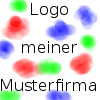
\includegraphics{images/cover/logo-company.png}}}
	\end{longtable}
	\enlargethispage{20mm}
	\begin{center}
    \doublespacing{
		\vspace*{12mm}	{\LARGE\textbf \documentTitle }}\\
		\vspace*{12mm}	{\large\textbf \documentType}\\
		\vspace*{12mm}	\degreePhrase\\
		\vspace*{3mm}		{\textbf \degree}\\
		\vspace*{12mm}	\departmentPhrase{} \department\\
    \vspace*{0mm}		\locationUniversityPhrase{} \locationUniversity\\
		\vspace*{12mm}	\documentAuthorPhrase\\
		\vspace*{3mm}		{\large\textbf \documentAuthor}\\
		\vspace*{12mm}	\releaseDate\\
	\end{center}
	\vfill
	\begin{spacing}{1.2}
	\begin{tabbing}
		mmmmmmmmmmmmmmmmmmmmmmmmmm             \= \kill
		\textbf{\documentPeriodPhrase}       \>  \documentPeriod\\
		\textbf{\matriculationNumberPhrase, \coursePhrase}  \>  \matriculationNumber, \course\\
		\textbf{\companyPhrase}                  \>  \companyName, \companyLocation\\
		\textbf{\tutorPhrase}               \>  \tutor\\
		\textbf{\evaluatorPhrase}              \>  \evaluator
	\end{tabbing}
	\end{spacing}
\end{titlepage}

	\end{spacing}
	\newpage

	\pagenumbering{Roman}

	% Restriction notices
	\ifDocType{T2\_3100}{%
		% no restricition notices for semester paper
	}{%
		%!TEX root = ../main.tex

\thispagestyle{empty}

\section*{\restrictionNoticesPhrase}

\vspace*{2em}

\iflang{de}{%
  Die vorliegende {\documentTypePhrase} mit dem Titel {\itshape{} \documentTitle{}\/} enthält 
  unternehmensinterne bzw. vertrauliche Informationen der {\companyName}, ist deshalb mit einem 
  Sperrvermerk versehen und wird ausschließlich zu Prüfungszwecken am Studiengang {\department} 
  der Dualen Hochschule Baden-Württemberg {\locationUniversity} vorgelegt. Sie ist ausschließlich zur 
  Einsicht durch den zugeteilten Gutachter, die Leitung des Studiengangs und ggf. den Prüfungsausschuss 
  des Studiengangs bestimmt.  Es ist untersagt,
  \begin{itemize}
  \item den Inhalt dieser Arbeit (einschließlich Daten, Abbildungen, Tabellen, Zeichnungen usw.) als 
            Ganzes oder auszugsweise weiterzugeben,
  \item Kopien oder Abschriften dieser Arbeit (einschließlich Daten, Abbildungen, Tabellen, 
             Zeichnungen usw.) als Ganzes oder in Auszügen anzufertigen,
  \item diese Arbeit zu veröffentlichen bzw. digital, elektronisch oder virtuell zur Verfügung zu stellen. 
  \end{itemize}
Jede anderweitige Einsichtnahme und Veröffentlichung – auch von Teilen der Arbeit – bedarf der 
vorherigen Zustimmung durch den Verfasser und {\companyName}.
}

%http://www.ib.dhbw-mannheim.de/fileadmin/ms/bwl-ib/Downloads_alt/Leitfaden_31.05.pdf

\iflang{en}{%
  The {\documentTypePhrase} on hand
  \begin{center}{\itshape{} \documentTitle{}\/}\end{center}
   contains internal resp.\ confidential data of {\companyName}. It is intended solely for inspection by the
   assigned examiner, the head of the {\department} department and, if necessary, the Audit
   Committee \locationUniversityPhrase{} {\locationUniversity}. It is strictly forbidden
    \begin{itemize}
    \item to distribute the content of this paper (including data, figures, tables, charts etc.) as a whole or 
              in extracts,
    \item to make copies or transcripts of this paper or of parts of it,
    \item to display this paper or make it available in digital, electronic or virtual form.
    \end{itemize}
  Exceptional cases may be considered through permission granted in written form by the author 
  and {\companyName}.
}

\vspace{3em}

\releaseLocation, \releaseDate
\vspace{4em}

\rule{6cm}{0.4pt}\\
\documentAuthor

		\newpage
	}%

	% Declaration
	%!TEX root = ../main.tex

\thispagestyle{empty}

\vspace*{2cm}
\section*{\declarationPhrase}

\vspace*{2em}

\iflang{de}{%
  gemäß Ziffer 1.1.13 der Anlage 1 zu §§ 3, 4 und 5  der Studien- und Prüfungsordnung für die Bachelorstudiengänge im Studienbereich Technik der Dualen Hochschule Baden-Württemberg vom 29.09.2017.

  \ifMultipleAuthors{Wir versichern}{Ich versichere} hiermit, dass \ifMultipleAuthors{wir unsere}{ich meine} 
  {\documentTypePhrase}mit dem Thema:
  \begin{center}
    {\textsf \documentTitle }
  \end{center}
  selbstständig verfasst und  keine anderen als die angegebenen Quellen und Hilfsmittel benutzt \ifMultipleAuthors{haben}{habe}. 
  \ifMultipleAuthors{Wir versichern}{Ich versichere} zudem, dass die eingereichte elektronische Fassung mit der gedruckten Fassung 
  übereinstimmt. 
}


\iflang{en}{%
  Hereby \ifMultipleAuthors{we}{I} solemnly declare:
  \begin{enumerate}
  \item that this {\documentTypePhrase}, titled {\itshape \documentTitle } is entirely the product of \ifMultipleAuthors{our}{my} 
            own scholarly work, unless otherwise indicated in the text or references, or acknowledged below;
  \item \ifMultipleAuthors{we}{I} have indicated the thoughts adopted directly or indirectly from other sources at the appropriate 
            places within the document;
  \item this {\documentTypePhrase} has not been submitted either in whole or part, for a degree at this or 
            any other university or institution;
  \item \ifMultipleAuthors{we}{I} have not published this {\documentTypePhrase} in the past;
  \item the printed version is equivalent to the submitted electronic one.
  \end{enumerate}
  \ifMultipleAuthors{We are}{I am} aware that a dishonest declaration will entail legal consequences.
}

\vspace{3em}

\releaseLocation, \iflang{de}{den}\iflang{en}{the} \releaseDate
\vspace{4em}

\rule{6cm}{0.4pt}\\
\documentAuthor

	\newpage

	% Abstract
	%!TEX root = ../dokumentation.tex

\pagestyle{empty}

% override abstract headline
\renewcommand{\abstractname}{Abstract}

\begin{abstract}

\end{abstract}
	\newpage

        % only page number in footer
	\pagestyle{plain}
	
	% space bevore chapter headline
	\RedeclareSectionCommand[beforeskip=\chapterMargin]{chapter}

	% Contents
	\begin{spacing}{1.1}
		\begingroup
		
		    % set subchapter depth
			\setcounter{tocdepth}{2}
			
			\tableofcontents
			\clearpage
		\endgroup
	\end{spacing}
	\newpage

	% Acronyms
	\cleardoublepage
    %!TEX root = ../dokumentation.tex

\addchap{\acronymsPhrase}

\begin{acronym}[YTMMM]
\setlength{\itemsep}{-\parsep}

\acro{AGPL}{Affero GNU General Public License}

\end{acronym}


	% List of Figures
	\cleardoublepage
	\listoffigures

	%List of Tables
	\cleardoublepage
	\listoftables

	% List of Listings
	\cleardoublepage
	\lstlistoflistings
	\cleardoublepage

	\pagenumbering{arabic}
	
	\pagestyle{headings}

	%Content
	\foreach \i in {01,02,03,04,05,06,07,08,09,...,99} {%
		\edef\FileName{content/chapter/\i .tex}%
			\IfFileExists{\FileName}{%
				\input{\FileName}
			}
			{%
%				No chapter available
			}
	}

	\clearpage

	% Bibilography
	\cleardoublepage
	\printbibliography

	% Glossar
	\cleardoublepage
	\printglossary[style=altlist,title=\glossaryPhrase]
	%!TEX root = ../main.tex

%
% To create glossary run the following command: 
% makeglossaries main.acn && makeglossaries main.glo
%

%
% Glossareintraege --> referenz, name, beschreibung
% Aufruf mit \gls{...}
%
\newglossaryentry{Glossareintrag}{name={Glossareintrag},plural={Glossareinträge},description={Ein Glossar beschreibt verschiedenste Dinge in kurzen Worten}}

	
	% Appendix
	\clearpage
	\appendix
	% !TeX root = ../dokumentation.tex

\addchap{\langanhang}



	
\end{document}
